\chapter{Details of model creation and computing}
\section{Rover3D model creation with Maple}

A Maple code package will be created to generate the dynamical system of the Rover %(in the  figure). 
and C files for visualization.


\subsection{Kinematic data and Geometry description of Rover}

We used the Cardan representation for the Rover model.\\

% insert the coordinate system figures.

The description of the dynamical data of the Rover is composed with "solids". "Solids" are linked with each other using vectors. An $(O_k, X_k, Y_k, Z_k)$ frame is attached to each solid $k$. The position and the orientation of the frame $k$ is given in the frame $ref_k$ of the solid it is attached to. So we need six parameters to describe a new "solid". A translation $(Tx_k, Ty_k, Tz_k)$ and a rotation of $z_k$ around
$z_{ref_k}$ (roll), a rotation of $y_k$ around the resulting $y$-axis (pitch) and finally a rotation of $x_k$ around the resulting $x$-axis
(yaw) should be included in the Dynamical data file for Maple code. \\

The figure \eqref{RoverSketup} will show us the geometry of Rover and describes what is "solids" and relationship between each other. A part of the \textbf{KinematicData.maple} input file is given to illustrate the structure of the dynamic data description. \footnote{The 3D model file in Google Sketchup format could found in: /home/bipop/jyang/siconos/trunk/SandBox/Rover}\\

\begin{figure}[H]
 \begin{center}
      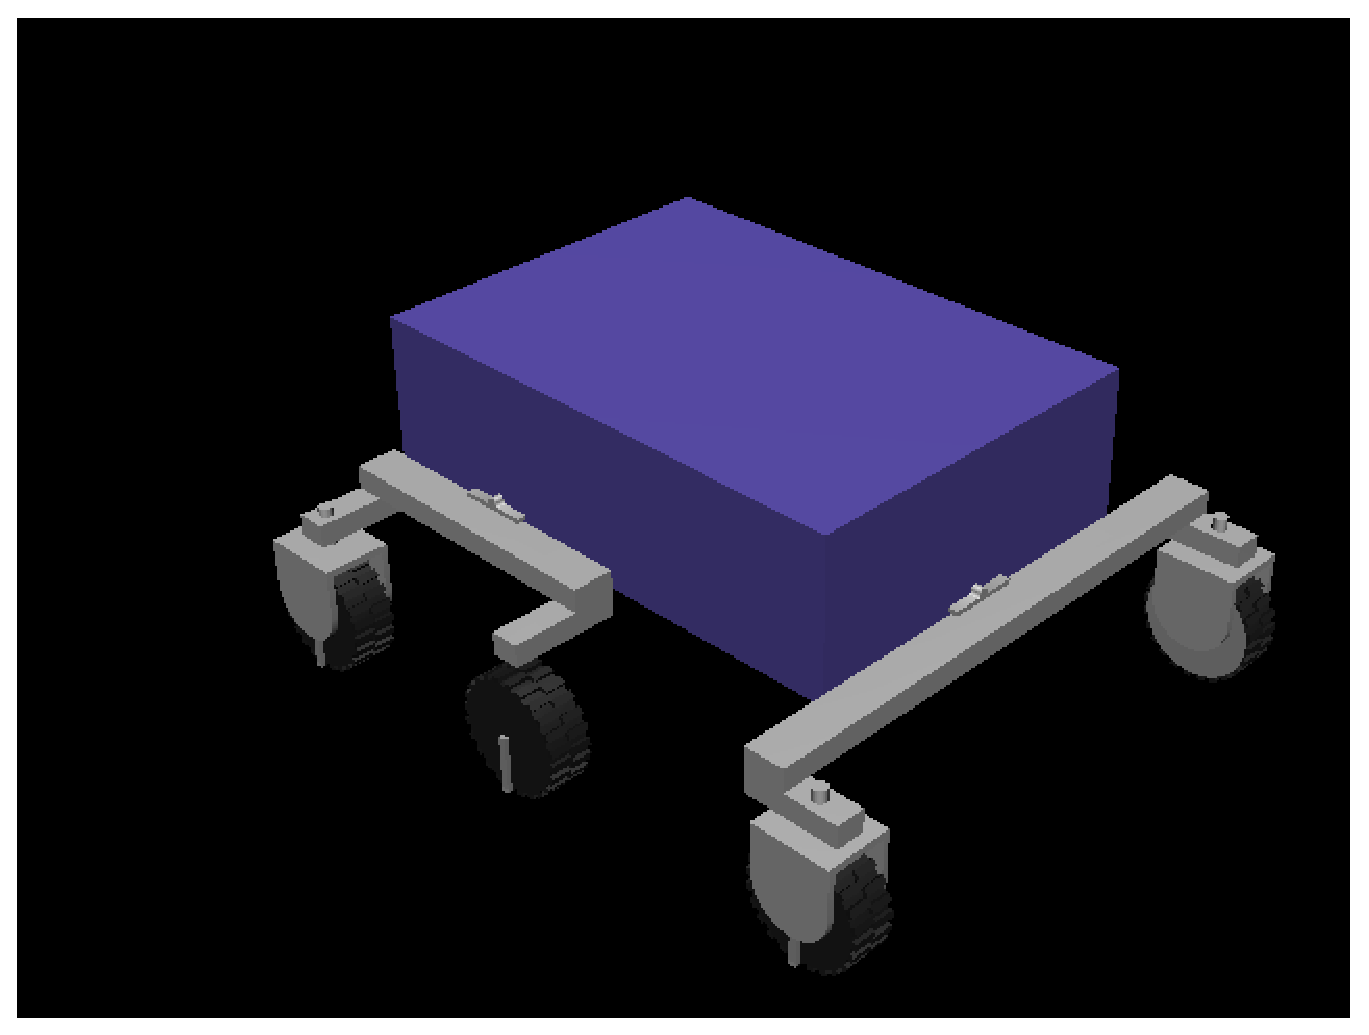
\includegraphics[width=3in]{Chapter4/rovereps.eps}
    \caption{Geometry of Rover}
  \end{center}
\label{RoverSketup}
\end{figure}


% insert the kinematic system figures.
\begin{figure}
\begin{center}
 \input{Chapter4/kinematic1.pstex_t}
\caption{Articular notations of Rover}
\end{center}
\end{figure}


\begin{figure}[!h]
\begin{minipage}[t]{.6\linewidth}
\begin{center}
\begin{tiny}
\begin{verbatim}
# solids number
NSOL := 16:

# degrees of freedom number
NDDL := 21:

#generalized coordinates and velocity definition
q := vector(NDDL):
qdot := vector(NDDL):

# l = vector of mechanical lenghts


#Cardan Rotation: We begin with the rotation around z, then around y then
#around x

# Frame 1 : Mass center: Orientation and position
ref_1	:= 0:
z_1 := q[6]:   #rotation along x,y,z aixs
y_1 := q[5]:
x_1 := q[4]:
Tx_1 := q[1]:  #location of the rover
Ty_1 := q[2]:
Tz_1 := q[3]:

# Frame 2 : Axle F (Front)
ref_2	:= 1:
z_2	:= 0:
y_2	:= 0:
x_2	:= q[7]:  #have a rotation freedom in x direction
Tx_2	:= 62:    #translation vector from its reference solid (solid 1)
Ty_2	:= -10:  
Tz_2	:= 0:

# Frame 3 : Steering Axle FL (Front Left)
ref_3	:= 2:
z_3	:= 0:
y_3	:= q[8]:  #Have a roataion degree of freedom in y direction
x_3	:= 0:    
Tx_3	:= 0:     #translation vector from its reference solid(Solid 2)
Ty_3	:= 0:
Tz_3	:= -53:

.
.
.
\end{verbatim}
\end{tiny}
\end{center}
\end{minipage}
\hfill
\begin{minipage}[t]{.4\linewidth}
\begin{center}
\begin{tiny}
\begin{verbatim}
.
.
.

# Frame 14 : Steering Axle BR 
ref_14	:= 12:
z_14	:= 0:
y_14	:= q[19]:
x_14	:= 0:
Tx_14	:= -30:
Ty_14	:= 0:
Tz_14	:= 0:

# Frame 15 : Wheel MR 
ref_15	:= 13:
z_15	:= q[20]:
y_15	:= 0:
x_15	:= 0:
Tx_15	:= 0:
Ty_15	:= -15:
Tz_15	:= 0:

# Frame 16 : Wheel BR 
ref_16	:= 14:
z_16	:= q[21]:
y_16	:= 0:
x_16	:= 0:
Tx_16	:= 0:
Ty_16	:= -15:
Tz_16	:= 0:

\end{verbatim}
\end{tiny}
\end{center}
\end{minipage}
\caption{Part of \textbf{KinematicData.maple} file which describes the
  position and the orientation of a jointed model with the
  yaw-pitch-roll angles.}
\label{fig:LagMod-CarAngKinematicData}
\end{figure}

With \textbf{KinematicData.maple}, the maple code knows the translation and rotation information between nodes. The table will describe all the name of nodes(Solids) and its degree of freedom and location in local frame.
 
\newcommand{\tabincell}[2]{\begin{tabular}{@{}#1@{}}#2\end{tabular}}
\begin{table}[htbp]
\begin{center}
\begin{tabular}{lccccc}
  \toprule
   No. & Name   & Ref. No. & \tabincell{c}{Rotation\\freedom} & \tabincell{c}{Location in\\Ref fram} & Description\\
  \midrule
  1 &Mass center & Non & $x,y,z$ & $(0,0,0)$ & \tabincell{c}{The mass center\\of the Rover, 6 DOF}\\
  2&Axle F  & 1 &  $x$ & $(62,-10,0)$ & The pivot at the front \\
  3&\tabincell{c}{Steering\\ Axle FL} & 2 & $y$ & $(0,0,-53)$ & \tabincell{c}{Steering Axle\\ at the front left side}\\
  4&\tabincell{c}{Steering\\ Axle FR} & 2 & $y$ & $(0,0,53)$ & \tabincell{c}{Steering Axle\\ at the front right side}\\
  5&Wheel FL & 3 & $z$ & $(0,-15,0)$ & \tabincell{c}{Rover Tire at the\\ front left side}\\
  6&Wheel FR & 4 & $z$ & $(0,-15,0)$ & \tabincell{c}{Rover Tire at the\\ front right side}\\
  7&Axle BL  & 1 &  $z$ & $(-40,-10,-53)$ & \tabincell{c}{The pivot at\\ left side} \\
  8&\tabincell{c}{Steering\\ Axle ML} & 7 & $y$ & $(30,0,0)$ & \tabincell{c}{Steering Axle at\\the middle of left side}\\
  9&\tabincell{c}{Steering\\ Axle BL} & 7 & $y$ & $(-30,0,0)$ & \tabincell{c}{Steering Axle at\\the back of left side}\\
  10&Wheel ML & 8 & $z$ & $(0,-15,0)$ & \tabincell{c}{Rover Tire at the\\middle of left side}\\
  11&Wheel BL & 9 & $z$ & $(0,-15,0)$ & \tabincell{c}{Rover Tire at the\\back of left side}\\
  12&Axle BR  & 1 &  $z$ & $(-40,-10,53)$ & \tabincell{c}{The pivot at\\ right side} \\
  13&\tabincell{c}{Steering\\ Axle MR} & 12 & $y$ & $(30,0,0)$ & \tabincell{c}{Steering Axle at\\the middle of right side}\\
  14&\tabincell{c}{Steering\\ Axle BR} & 12 & $y$ & $(-30,0,0)$ & \tabincell{c}{Steering Axle at\\the back of right side}\\
  15&Wheel MR & 13 & $z$ & $(0,-15,0)$ & \tabincell{c}{Rover Tire at the\\middle of right side}\\
  16&Wheel BR & 14 & $z$ & $(0,-15,0)$ & \tabincell{c}{Rover Tire at the\\back of right side}\\


  \bottomrule
 \end{tabular}
\caption{Kinematic Data of the Rover}
\end{center}
\end{table}


Some characteristic points which we are interested could be defined as tags. We create a maple file \textbf{AdditionnalData.maple} to describe the location of Tags. The data describing location tags could be composed as two part: 
\begin{itemize}
\item The Number of Ref solid the tag is attached to
\item One vector describing the translation from this Solid point
\end{itemize}

\begin{figure}[!h]
\begin{minipage}[t]{.6\linewidth}
\begin{center}
\begin{tiny}
\begin{verbatim}
# Definition de quelques points importants (tags)

# Tag 1 : Mass center
reftag_1 := 1:           #Ref Number which the tag is attached to
tag_1    := vector([0,0,0]):  #vector from this Solid

# Tag 2 : Pivot F
reftag_2 := 2:
tag_2    := vector([0,0,0]):
.
.
.

\end{verbatim}
\end{tiny}
\end{center}
\end{minipage}
\caption{Part of \textbf{AdditionnalData.maple} file which describes the
  positions of the tags in their attached segment frame.}
\label{fig:LagMod-AdditionnalData}
\end{figure}


The main Maple code \textbf{ModelGeneration.maple} will generate a C file \textbf{Tags.c} with the data in \textbf{AdditionnalData.maple}.
This C file enable us to get the global coordinate data of all the Tags. In order to use this C file to compute the coordinates. We need to input the state vector q as well as a null matrix T which will be used for output. \\

$T$ is on the form:
$$
T = 
\left(
\begin{array}{ccc}
x_{tag_1}^{0} & y_{tag_1}^{0} & z_{tag_1}^{0} \\
x_{tag_2}^{0} & y_{tag_2}^{0} & z_{tag_2}^{0} \\
\vdots & \vdots & \vdots \\
x_{tag_{NumberOfTags}}^{0} & y_{tag_{NumberOfTags}}^{0} &
z_{tag_{NumberOfTags}}^{0} \\
x_{CenterOfMass}^{0} & y_{CenterOfMass}^{0} & z_{CenterOfMass}^{0} \\
\end{array}
\right)
$$
where the $0$ represents the reference frame. 

\subsection{Dynamical data input}
The inertials parameters (the gravity vector, the mass of the segment, the position of
the segments centers of mass and the inertia matrix of these segments
relative to the centers of their attached frames) are defined in the file \textbf{DynamicData.maple}. The
figure \ref{fig:LagMod-DynamicData} shows an example of this file. 

\begin{figure}[H]
\begin{minipage}[t]{.6\linewidth}
\begin{center}
\begin{tiny}
\begin{verbatim}

#dynamic data for Rover3D

# Gravity vector
Gravity := vector([0, -9.81, 0]):


# solid size matrix (a,b,c) on (x,y,z) in meters unity
sizematrix := [[120,40,100], #  trunk: Orientation and position
               [6,6,115],    #  Axle F (Front) 			
               [3,15,0],     #	Steering Axle FL (Front Left)	
               [3,15,0],     #  Steering Axle FR (Front Right)	
               [10,0,0],     #  Wheel FL		
               [10,0,0],     #  Wheel FR			
               [70,6,6],     #  Axle BL				
               [3,15,0],     #  Steering Axle ML  		
               [3,15,0],     #  Steering Axle BL  	
               [10,0,0],     #  Wheel ML 			
               [10,0,0],     #  Wheel BL 			
               [70,6,6],     #  Axle BR
               [3,15,0],     #  Steering Axle MR 		
               [3,15,0],     #  Steering Axle BR 		
               [10,0,0],     #  Wheel MR       			
               [10,0,0]]:    #	Wheel BR       			


# Rover total mass in kilogrammes unity
Mass := 1:	


# solid mass matrix in rate of total mass
massmatrix := [600,   #  trunk: Orientation and position
               50,    #  Axle F (Front)
               5,     #	 Steering Axle FL (Front Left)
               5,     #  Steering Axle FR (Front Right)
               30,    #  Wheel FL
               30,    #  Wheel FR
               50,    #  Axle BL
               5,     #  Steering Axle ML 
               5,     #  Steering Axle BL 
               30,    #  Wheel ML
               30,    #  Wheel BL 
               50,    #  Axle BR
               5,     #  Steering Axle MR 
               5,     #  Steering Axle BR 
               30,    #  Wheel MR 
               30]*1:   #	 Wheel BR 

MatHuygens := proc(G) option remember;

	RETURN(matrix([[G[3]^2+G[2]^2, -G[2]*G[1], -G[3]*G[1]],
		[-G[2]*G[1], G[3]^2+G[1]^2, -G[3]*G[2]],
		[-G[3]*G[1], -G[3]*G[2], G[2]^2+G[1]^2]])):
end:


# function created to compute the inertia matrix

IOMatrix := proc(k) option remember;
local mk, IG, Gk;
	
	mk := Mass * massmatrix[k]:
	IG := matrix([[mk*(sizematrix[k,3]^2 + sizematrix[k,2]^2) /12, 0, 0],
		      [0, mk*(sizematrix[k,1]^2 + sizematrix[k,3]^2) /12, 0],
		      [0, 0, mk*(sizematrix[k,1]^2 + sizematrix[k,2]^2) /12]]):
	Gk := G_||(k):
	RETURN(evalm(IG + mk*MatHuygens(Gk))):	
end:


.
.
.
\end{verbatim}
\end{tiny}
\end{center}
\end{minipage}
\hfill
\begin{minipage}[t]{.4\linewidth}
\begin{center}
\begin{tiny}
\begin{verbatim}
.
.
.

#Inertia matrix for Disk
IOMatrixDisk :=proc(k) option remember;
local mk , r, IG;
      mk := Mass*massmatrix[k]:
      r  := sizematrix[k,1]:
      IG := matrix([[mk*r^2/4, 0, 0],
		      [0,mk*r^2/4, 0],
		      [0, 0,mk*r^2/2 ]]):
      RETURN(IG):	
end:

#Inertia matrix for Cylinder
IOMatrixCylinder := proc(k) option remember;
local mk, r, h, IG;
       mk :=Mass*massmatrix[k]:
       r  := sizematrix[k,1]:
       h  := sizematrix[k,2]:
       IG := matrix([[mk*(3*r^2+h^2)/12,0,0],
                     [0,mk*r^2/2,0],
                     [0,0,mk*(3*r^2+h^2)/12]]):
       RETURN(IG):
end:


# Solid 1 : trunk: Orientation and position
m_1  := massmatrix[1]*Mass:
G_1  := vector([0, 0, 0]):
IO_1 := IOMatrix(1):


# Solid 2 : Axle F (Front)
m_2  := massmatrix[2]*Mass:
G_2  := vector([0, 0, 0]):
IO_2 := IOMatrix(2):


# Solid 3 : Steering Axle FL (Front Left)
m_3  := massmatrix[3]*Mass:
G_3  := vector([0, 0, 0]):
IO_3 := IOMatrixCylinder(3):


# Solid 4 : Steering Axle FR (Front Right)
m_4  := massmatrix[4]*Mass:
G_4  := vector([0, 0, 0]):
IO_4 := IOMatrixCylinder(4):


# Solid 5 : Wheel FL
m_5  := massmatrix[5]*Mass:
G_5  := vector([0, 0, 0]):
IO_5 := IOMatrixDisk(5):


# Solid 6 : Wheel FR
m_6  := massmatrix[6]*Mass:
G_6  := vector([0, 0, 0]):
IO_6 := IOMatrixDisk(6):



\end{verbatim}
\end{tiny}
\end{center}
\end{minipage}
\caption{The \textbf{DynamicData.maple} file describes different
  inertial parameters of the model.}
\label{fig:LagMod-DynamicData}
\end{figure}

In this maple file, we could define:

\begin{itemize}
\item The gravity vector (defined in vector Gravity)
\item The geometry of every segment (defined in Matrix sizematrix, length, height,width,radius etc)
\item Mass of each segment (defined in the Matrix massmatrix)
\item Mass center of the segment (defined in \verb|G_i|, i is the solid number), and the function MatHuygens will be called to do the translation if the mass center is not at the geometry center.
\item Inertia matrix is defined in the function IOMatrix,IOMatrixDisk,IOMatrixCylinder, which are for inertia matrix computing of rectangle,disk and cylinder respectively.
\end{itemize}

The \textbf{ModelGeneration.maple} file contains:

\begin{itemize}
\item \textbf{GenerateInertiaMatrix} procedure which uses the \textbf{InertiaRecursion} function to generate the \textbf{Inertia.c}
file.
\item \textbf{GenerateNLEffectsVector} procedure which uses the \textbf{NLEffectsRecursion} function to generate the
\textbf{NLEffects.c} file
\end {itemize}


\chapter{Contact Description}

To describe the contact of the Rover with the solid ground or granular soil in Siconos, we need two plugin functions:
\begin{itemize}
\item $h$ function to compute the distance between contact points
\item $G$ is the transformation matrix of velocity of contact points from the global frame to the local frame
\end{itemize}
To simplify the model, we only consider point contact. In this contact model, we simplify the axis of the wheel into a point, and create contact model between this point and the sphere or plane.
  

\section{Computation of distance}
\subsection{Wheel/Plane Contact}
With the use of Tags.c file, we can get all the coordinates of tags. In \textbf{AdditionnalData.maple}, we set some points on the tyres as tags, from which we can get the coordinates. Consider tyre plane contact in Fig \eqref{WHcontact}, $E$ is the contact point. Assume the plane equation is $Ax+By+Cz+D=0$, the length of line $EF$ is the distance we want for the contact model.

\begin{figure}[H]
\begin{center}
 \input{Chapter4/contactplane.pstex_t}
\caption{Wheel/Plane Contact}
\label{WHcontact}
\end{center}
\end{figure}

The algorithm for computing distance could be summarized as flowing steps.

\begin{itemize}
\item Vector $\vec{s}$ is a unit vector perpendicular to the tyre. In order to get this vector, we set this vector as a tag in \textbf{AdditionnalData.maple}. Then it is possible to obtain this vector from \textbf{Tags.c}.
\item Vector $\vec{n}_{plane}$ is a vector perpendicular the plane. It is obtained from the plane equation $Ax+By+Cz+D=0$: $\vec{n}_{plane}=(A,B,C)$
\item The vector pointing the moving direction of tyre $\vec{m}$ could be obtained by cross product of  $\vec{s}$ and $\vec{n}_{plane}$, $\vec{m}=\vec{n}_{plane} \times \vec{s}$
\item Vector $\vec{t}$ is the normalized vector of $\vec{m}$.
\item The normal vector of local frame $\vec{n}$ could be obtained from the cross product of $\vec{t}$ and $\vec{s}$: $\vec{n}=\vec{s} \times \vec{t}$.
\item The vector pointing to the contact point $\overrightarrow{GE}=-R\vec{n}$. Where $R$ is the radius of the tyre.
\item The coordinates of contact point $E$ could be obtain by vector operation: $\overrightarrow{OE}=\overrightarrow{OG}+\overrightarrow{GE}$.
\item The value of distance could be obtained by using distance formulation \eqref{DistanceFormulation} 
\end{itemize}


\begin{eqnarray}
d= \frac{\left| Ax+By+Cz+D \right|}{\sqrt{A^2+B^2+C^2}}
\label{DistanceFormulation}
\end{eqnarray}

We make a function $ContactDistance$ in \textbf{ModelGeneration.maple} to compute the distance of six contact points and save the result in a vector. The vector will be export as a C file \textbf{Distance.c}. To use this C file, we need to input the state vector $q$, and four parameter vector $P=(A,B,C,D)$ of the plane, as well as a Null vector $distance$ which the result will be saved to. The general format is \textbf{Distance(distance,P,q)}.\\

And during the computing of the contact distance, local frame is also obtained: $(\vec{s},\vec{t},\vec{n})$.

\subsection{Wheel/Sphere Contact}

\begin{figure}[H]
\begin{center}
 \input{Chapter4/contactsphere.pstex_t}
\caption{Wheel/Sphere Contact}
\label{Wheel/Sphere Contact}
\end{center}
\end{figure}


In Wheel/Sphere distance computation, flowing steps are used to obtain the contact distance.

\begin{itemize}
\item With similar method used in Wheel Plane contact, we can obtain the vector $\vec{s}$ which is perpendicular to the tyre by defining a tag in \textbf{AdditionnalData.maple}.
\item Assum $\vec{s}=(A,B,C)$ and the coordinates of point $D$ is $\overrightarrow{OD}=(x_0,y_0,z_0)$, we can write the tyre plane equation as $Ax+By+Cz=Ax_0+By_0+Cz_0$.
\item The distance between the sphere and the tyre plane $\left| \overrightarrow{AB} \right|$ could be obtained by formulation \eqref{DistanceFormulation}. 
\item \begin{eqnarray}
      &\overrightarrow{AB}=-\left| \overrightarrow{AB} \right| \overrightarrow{s}& \\
      &\overrightarrow{OB}=\overrightarrow{OA}+\overrightarrow{AB}& \\
      &\overrightarrow{DB}=\overrightarrow{OB}-\overrightarrow{OD}& \\
      &\overrightarrow{DC}=\frac{\overrightarrow{DB}}{\left| \overrightarrow{DB} \right|}R& \quad \text{where $R$ is the radius of the tyre}\\ 
      &\overrightarrow{OC}=\overrightarrow{OD}+\overrightarrow{DC}&
      \end{eqnarray}
\item With the coordinates of point $C$, the contact distance is obtained by $\left| \overrightarrow{OA}-\overrightarrow{OC} \right|-R_s \quad$ where $R_s$ is the radius of the sphere. 
\item What's more, we can obtain the local fram vector $\vec{n}=-\frac{\overrightarrow{DC}}{\left| \overrightarrow{DC} \right|}$ , $\vec{t}=\vec{n} \times \vec{s}$
\end{itemize}

\section{$G$ function computation}

To construct the local velocity frame, we need local coordinate system $(\vec{s},\vec{t},\vec{n})$ \\


With the local frame $(\vec{s},\vec{t},\vec{n})$, we could use matrix $[\vec{s},\vec{t},\vec{n}]$ as rotation matrix to transform the global velocity to local frame.\\

In order to get the velocity in local frame, we start from the global coordinates. Function ContactVector in \textbf{ModelGeneration.maple} could give the coordinates of contact points for us. They are functions of state vector $q$: 

\begin{eqnarray}
P_{global}=\begin{pmatrix}
x(q)\\
y(q)\\
z(q)
\end{pmatrix}
\end{eqnarray}

And we have velocity in global frame:

\begin{eqnarray}
v_{global}=\frac{dP_{global}}{dt}=
\begin{pmatrix}
\frac{dx(q)}{dt}\\
\frac{dy(q)}{dt}\\
\frac{dz(q)}{dt}
\end{pmatrix}=
\begin{pmatrix}
\nabla_{q}x\\
\nabla_{q}y\\
\nabla_{q}z
\end{pmatrix}\dot{q}
\end{eqnarray}

And we can get the velocity in local frame by multiplying the rotation matrix $T=[\vec{s},\vec{t},\vec{n}]$

\begin{eqnarray}
v_{local}=Tv_{global}=T\begin{pmatrix}
\nabla_{q}x\\
\nabla_{q}y\\
\nabla_{q}z
\end{pmatrix}\dot{q}=G\dot{q}
\end{eqnarray}

The matrix $G=T(\nabla_{q}x,\nabla_{q}y,\nabla_{q}z)^T$ is what we need in Siconos relation definition.

The computing procedure of matrix $G$ is in function ContactJacobianMatrix of file \textbf{ModelGeneration.maple}


\subsection{Consideration of thickness of the wheels}

The model for computing the distance is for the wheels without thickness, or very "thin" wheels. Now, we develop the model with consideration of thickness. \\


In the previous section, we have found the contact point of thin wheel, and assume the coordinates is $\overrightarrow{OA}$. We can prove that all the possible contact point $B$ on the wheel could be written as $\overrightarrow{OB}=\overrightarrow{OA}+k\vec{s}$, where $\vec{s}$ is the unite vector normal to the wheel plane. And $-\frac{t}{2}\le k \le \frac{t}{2}, \quad t \quad \text{is the thickness of the wheel}$.

\begin{figure}[H]
\begin{center}
 \input{Chapter4/thickness.pstex_t}
\caption{Model with consideration of thickness}
\label{Thickness}
\end{center}
\end{figure}

And function $f(\overrightarrow{OB})$ compute the distance between the contact points. The contact distance with consideration of thickness could be written as: $h(q)=minimize_{k} \quad f(\overrightarrow{OB}=\overrightarrow{OA}+k\vec{s})$.\\

In the Maple software, the computing time of analytical solution is not acceptable. A numerical approximation is implemented in the code. We export the analytical solution of distance $f(\overrightarrow{OA}+k\vec{s})$ in C file. In this C file, $k$ is keep as symbol. In the C++ class \textbf{Rover3DWheelFixedSphereR}, the interval $-\frac{t}{2}\le k \le \frac{t}{2}$ is divided into smaller intervals with same size. We only compute distances these points with spheres, and the shortest distances is selected as the contact distance.


\begin{equation}
h(q)= \underset{-\frac{t}{2}\le k \le \frac{t}{2}}{\text{minimize}}\quad f(\overrightarrow{OB}=\overrightarrow{OA}+k\vec{s})
\end{equation}


Where $k$ is the thickness of the wheel.
\section{PID controller}



A PID controller(proportional–integral–derivative controller) is used for the steering system of the rover.
Siconos enable us to put PID controller easily by plugging a external force term  $F_{Ext}(t,z)$ in the Lagrangian Non Linear Dynamical System. \ref{LNLDS}

\begin{equation}
M(q,z)\ddot{q}+NNL(\dot{q},q,z)+F_{Int}(\dot{q},q,t,z)=F_{Ext}(t,z)+p
\label{LNLDS}
\end{equation}

A typical PID control scheme is composed with three correcting terms in order to minimize the difference between  process variable(SP) and setpoint (PV):
\begin{equation}
MV(t)= P_{out} +I_{out}+ D_{out}
\end{equation}

Where 
\begin{eqnarray}
&P_{out}=K_pe(t)& \\
&I_{out}=K_i\int_0^{t} e(\tau) d\tau&\\
&D_{out}=K_d\frac{d}{dt}e(t)&\\
&K_p,K_i,K_d \quad& \text{tuning parameters}\\
&e(t)=SP-PV& \text{Error}
\end{eqnarray}

In our particular case, we only use two correcting terms $P_{out}$ and $D_{out}$:
\begin{eqnarray}
&P_{out}=K_p(q(i)-q_0(i))&\\
&D_{out}=K_d(v(i)-v_0(i))&
\end{eqnarray}

Where $q(i)$ is the variable we would like control. $q_0(i)$ is the initial value.

Hence, The dynamical system could be describe as:
\begin{equation}
M(q,z)\ddot{q}+NNL(\dot{q},q,z)+F_{Int}(\dot{q},q,t,z)=K_p(q(i)-q_0(i))+K_d(v(i)-v_0(i))+p
\label{LNLDSPID}
\end{equation}

The code for PID controller is include in the file  \textbf{RobotPlugin.cpp}
 


\section{Other useful functions}

To visualize the result in 3D, we need to create a VRML file with the result data. The VRML file use Axis angle rotation representation to describe a rotation, we need to transform our rotation matrix to an axis angle rotation representation when writing the VRML file.This procedure could be found in file \textbf{AdditionnalData.maple}.











